\newpage
\section{Conclusion}
\subsection{Conclusion}
The Big Data Auto-Tuning tool has been implemented as a fully integrated solution to finding optimum configuration for big data applications. It consists of a neat user interface in the Eclipse IDE, integrated to a Jenkins server running the BO4CO configuration optimisation tool, that deploys and monitors experiments on a Storm cluster, and retrieves results to the developer on the Eclipse plugin UI.\\
In doing so, the project has overcome challenges to achieve:
\begin{itemize}
\item -	A development environment in the Eclipse IDE, where developers can explore configuration optimisation and the performance of their applications.
	\begin{itemize}
	\item A new SWT-based widget, MultiSelectionCombo, that conforms to conventions and standards, and has been published to the open source community
    \item Extension to the BO4CO code to further this state of the art configuration optimisation tool to support Categoric and Boolean parameters in addition to numerical parameters
	\end{itemize}
\item -	Fully integrated development environment that triggers configuration optimisation on remote automation server and run tests on remote testbed.
	\begin{itemize}
	\item Integration between Eclipse and Jenkins for triggering parameterised builds with configuration files remotely, providing an example that integration between the two can be deeper and cover more advanced functionality than existing solutions.
    \item Integrated Jenkins automation server and MATLAB-based BO4CO tool, demonstrating a new viable continuous integration path for MATLAB and Jenkins on Windows-based systems.
	\end{itemize}
\end{itemize}

\newpage
\subsection{Future Works}
Future works relating to this project can explore the following directions:
\begin{itemize}
\item Big data framework configuration parameters\\
The criteria for inclusion of configuration parameters for this project can be improved with a better understanding of the underlying big data frameworks, and how the parameters are designed to affect operations. There can be more experimentation to collect statistics and more scientifically determine whether a configuration parameter would affect performance of big data applications. This data can also be used to better present the available parameters, by ordering and sorting them for different use cases, providing helpful hints to developers with less knowledge, and provide realistic limits and guideline figures to aid selection.
\item Extra features on the Eclipse plugin\\
	\begin{itemize}
    \item Improved visualisation and analysis of results - Configuration optimisation results can be accompanied with statistics to show how performance has improved over experiment runs.
	\item Saved session and settings - Frequently used settings can be saved and loaded for convenience. The services and test settings usually stays the same across many configuration optimisation experiment runs, only with the parameters changed. The developer will not need to always re-enter such information.
	\end{itemize}
\item Further work on BO4CO configuration optimisation tool\\
	\begin{itemize}
	\item Complete testing for Hadoop big data framework - Fixes to the tool have not been tested on Hadoop
    \item Investigate the performance of configuration optimisation with categorical and boolean parameters - The new capability has been implemented but lacks sufficient testing to statistically validate its performance. There is every reason to believe that it will perform similarly to how it has done with numerical parameters, possibly with a less predictable performance at the initial iterations, but converging to optimal solution after the initial stage.
	\end{itemize}
\end{itemize}
\newpage
\subsection{Acknowledgements}
I would like to express my sincere gratitude to my supervisor, Dr Giuliano Casale. His guidance to shape the direction of the project, unwavering assistance in fixing the BO4CO tool, and deep knowledge in the project area was invaluable in making this project a success.\\
I would also like to thank Matej Artač for his kind assistance in setting up the numerous tools required; and my second marker, Dr Robert Chatley, for his helpful advice and suggesting new perspectives from which to evaluate the project.

\newpage
\section{Appendix}
\subsubsection{Parameters XML schema}
\begin{figure}[h]
\centering
\caption{Parameters XML schema.}
\label{fig:schema}
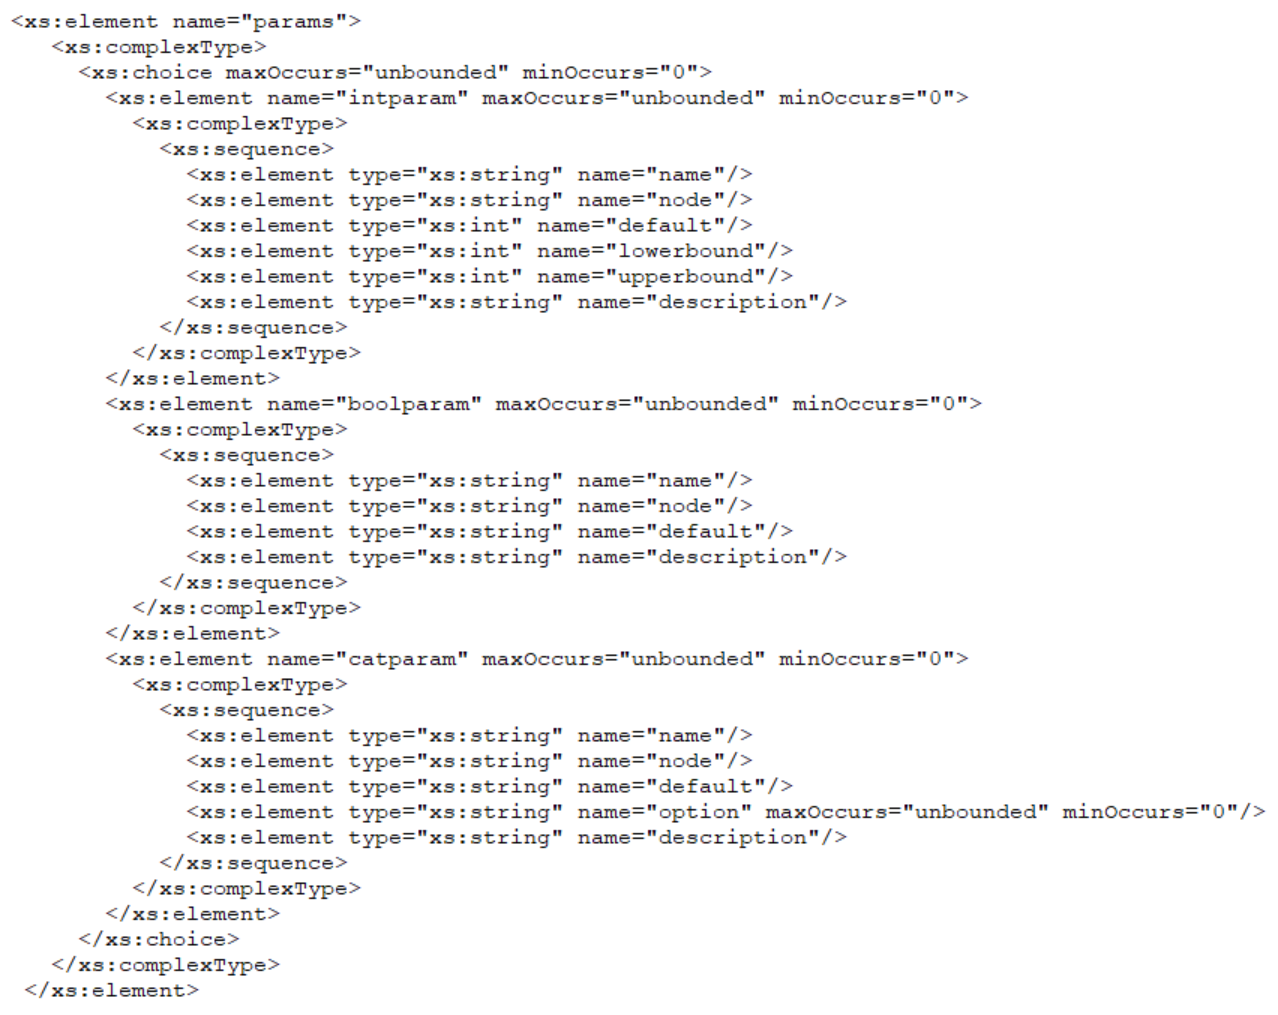
\includegraphics[width=\textwidth]{images/schema.png}
\end{figure}
\newpage
\subsubsection{Controls in SWT}
\cite{swtcontrol}
\begin{center}
\begin{tabular}{l|l}
Widget & Purpose\\
\hline
Browser & Control containing a native HTML renderer.\\
Button & Selectable control that issues notification when pressed and\/or released.\\
Canvas & \multirow{2}{*}{\parbox{12cm}{Composite control that provides a surface for drawing arbitrary graphics. Often used to implement custom controls.}}\\
& \\
Caret & An i-beam that is typically used as the insertion point for text.\\
Combo & \multirow{2}{*}{\parbox{12cm}{Selectable control that allows the user to choose a string from a list of strings, or optionally type a new value into an editable text field.}}\\
&\\
Composite & Control that is capable of containing other widgets.\\
CoolBar & \multirow{2}{*}{\parbox{12cm}{Composite control that allows users to dynamically reposition the cool items contained in the bar.}}\\
&\\
CoolItem & \multirow{2}{*}{\parbox{12cm}{Selectable user interface object that represents a dynamically positionable area of a cool bar.}}\\
&\\
DateTime & \multirow{2}{*}{\parbox{12cm}{Selectable user interface object that allows the user to enter and modify date or time values.}}\\
&\\
ExpandBar & \multirow{2}{*}{\parbox{12cm}{Composite control that groups pages that can be shown or hidden by the user with labeled headers.}}\\
&\\
ExpandItem & \multirow{2}{*}{\parbox{12cm}{Selectable user interface object corresponding to a header for a page in an ExpandBar.}}\\
&\\
Group & \multirow{2}{*}{\parbox{12cm}{Composite control that groups other widgets and surrounds them with an etched border and\/or label.}}\\
&\\
Label & Non-selectable control that displays a string or an image.\\
Link & Selectable control that displays a text with links.\\
List & \multirow{2}{*}{\parbox{12cm}{Selectable control that allows the user to choose a string or strings from a list of strings.}}\\
&\\
Menu & User interface object that contains menu items.\\
MenuItem & Selectable user interface object that represents an item in a menu.\\
ProgressBar & \multirow{2}{*}{\parbox{12cm}{Non-selectable control that displays progress to the user, typically in the form of a bar graph.}}\\
&\\
Sash & \multirow{3}{*}{\parbox{12cm}{Selectable control that allows the user to drag a rubber banded outline of the sash within the parent window. Used to allow users to resize child widgets by repositioning their dividing line.}}\\
&\\
&\\
Scale & Selectable control that represents a range of numeric values.\\
ScrollBar & \multirow{2}{*}{\parbox{12cm}{Selectable control that represents a range of positive numeric values. Used in a Composite that has V\_SCROLL and\/or H\_SCROLL styles.}}\\
&\\
Shell & \multirow{3}{*}{\parbox{12cm}{Window that is managed by the OS window manager. Shells can be parented by a Display (top level shells) or by another shell (secondary shells).}}\\
&\\
&\\
\end{tabular}
\end{center}
\begin{center}
\begin{tabular}{l|l}
Widget & Purpose\\
\hline
Slider & \multirow{3}{*}{\parbox{12cm}{Selectable control that represents a range of numeric values. A slider is distinguished from a scale by providing a draggable thumb that can adjust the current value along the range.}}\\
&\\
&\\
Spinner & \multirow{2}{*}{\parbox{12cm}{Selectable control that allows the user to enter and modify numeric values.}}\\
&\\
TabFolder & \multirow{2}{*}{\parbox{12cm}{Composite control that groups pages that can be selected by the user using labeled tabs.}}\\
&\\
TabItem & \multirow{2}{*}{\parbox{12cm}{Selectable user interface object corresponding to a tab for a page in a tab folder.}}\\
&\\
Table & \multirow{3}{*}{\parbox{12cm}{Selectable control that displays a list of table items that can be selected by the user. Items are presented in rows that display multiple columns representing different aspects of the items.}}\\
&\\
&\\
TableColumn & Selectable user interface object that represents a column in a table.\\
TableItem & Selectable user interface object that represents an item in a table.\\
Text & Editable control that allows the user to type text into it.\\
ToolBar & Composite control that supports the layout of selectable tool bar items.\\
ToolItem & Selectable user interface object that represents an item in a tool bar.\\
Tree & \multirow{2}{*}{\parbox{12cm}{Selectable control that displays a hierarchical list of tree items that can be selected by the user.}}\\
&\\
TreeColumn & Selectable user interface object that represents a column in a tree.\\
TreeItem & \multirow{2}{*}{\parbox{12cm}{Selectable user interface object that represents a hierarchy of tree items in a tree.}}\\
&\\
\end{tabular}
\end{center}

\subsubsection{Events in SWT}
\cite{swtevent}
\begin{center}
Low level events
\begin{tabular}{l|l}
Event Type & Description\\
\hline
FocusIn, FocusOut & A control has gained or lost focus.\\
KeyDown, KeyUp & \multirow{2}{*}{\parbox{10cm}{The user has pressed or released a keyboard key when the control has keyboard focus.}}\\
&\\
\multirow{2}{*}{\parbox{4.5cm}{MouseDown, MouseUp, MouseDoubleClick}} & \multirow{2}{*}{\parbox{10cm}{The user has pressed, released, or double clicked the mouse over the control.}}\\
&\\
MouseMove & The user has moved the mouse above the control.\\
\multirow{2}{*}{\parbox{4.5cm}{MouseEnter, MouseExit, MouseHover}} & The mouse has entered, exited, or hovered over the control.\\
&\\
\multirow{3}{*}{\parbox{4.5cm}{MouseHorizontalWheel, MouseVerticalWheel, MouseWheel}} & The mouse wheel has been rotated.\\
&\\
&\\
Paint & The control has been damaged and requires repainting.\\
Touch & \multirow{2}{*}{\parbox{10cm}{The user has touched a touch-based input source over the control.}}\\
&\\
\end{tabular}
\end{center}
\newpage
\begin{center}
High level events
\begin{tabular}{l|l}
Event Type & Description\\
\hline
Activate, Deactivate & Generated when a Control is activated or deactivated.\\
Arm & A MenuItem is armed (highlighted and ready to be selected).\\
Close & A Shell is about to close as requested by the window manager.\\
DefaultSelection & \multirow{2}{*}{\parbox{12cm}{The user selects an item by invoking a default selection action. For example, by hitting Enter or double clicking on a row in a Table.}}\\
&\\
Dispose & A widget is about to be disposed, either programmatically or by user.\\
DragDetect & The user has initiated a possible drag operation.\\
EraseItem & A TableItem or TreeItem is about to have its background drawn.\\
Expand, Collapse & An item in a Tree is expanded or collapsed.\\
Gesture & \multirow{2}{*}{\parbox{12cm}{The user has used a touch-based input source to perform a gesture over the control.}}\\
&\\
Help & \multirow{2}{*}{\parbox{12cm}{The user has requested help for a widget. For example, this occurs when the F1 key is pressed under Windows.}}\\
&\\
Iconify, Deiconify & A Shell has been minimized, maximized, or restored.\\
ImeComposition & \multirow{2}{*}{\parbox{12cm}{Allows custom text editors to implement in-line editing of international text.}}\\
&\\
MeasureItem & The size of a custom drawn TableItem or TreeItem is being requested.\\
MenuDetect & The user has requested a context menu.\\
Modify & The widget's text has been modified.\\
Move, Resize & \multirow{2}{*}{\parbox{12cm}{A control has changed position or has been resized, either programmatically or by user.}}\\
&\\
Movement & \multirow{2}{*}{\parbox{12cm}{An updated caret offset is needed in response to a user action in a StyledText.}}\\
&\\
OpenDocument & The operating system has requested that a document be opened.\\
OrientationChange & The orientation of a Text control is changing.\\
PaintItem & A TableItem or TreeItem is about to have its foreground drawn.\\
Selection & \multirow{3}{*}{\parbox{12cm}{The user selects an item in the control. For example, by single clicking on a row in a Table or by keyboard navigating through the items.}}\\
&\\
&\\
SetData & Data needs to be set on a TableItem when using a virtual table.\\
Settings & \multirow{2}{*}{\parbox{12cm}{An operating system property, such as a system font or color, has been changed.}}\\
&\\
Show, Hide & A control's visibility has changed.\\
Skin & A control needs to be skinned.\\
Traverse & \multirow{2}{*}{\parbox{12cm}{The user is trying to traverse out of the control using a keystroke. For example, the escape or tab keys are used for traversal.}}\\
&\\
Verify & \multirow{2}{*}{\parbox{12cm}{A widget's text is about to be modified. This event gives the application a chance to alter the text or prevent the modification.}}\\
&\\
\end{tabular}
\end{center}

\newpage
\printbibliography
